\item \underline{Correas Laterales.}\\
\begin{itemize}

\item El estado de carga corresponde a peso propio + viento.

\begin{figure}[H]
\begin{center}
     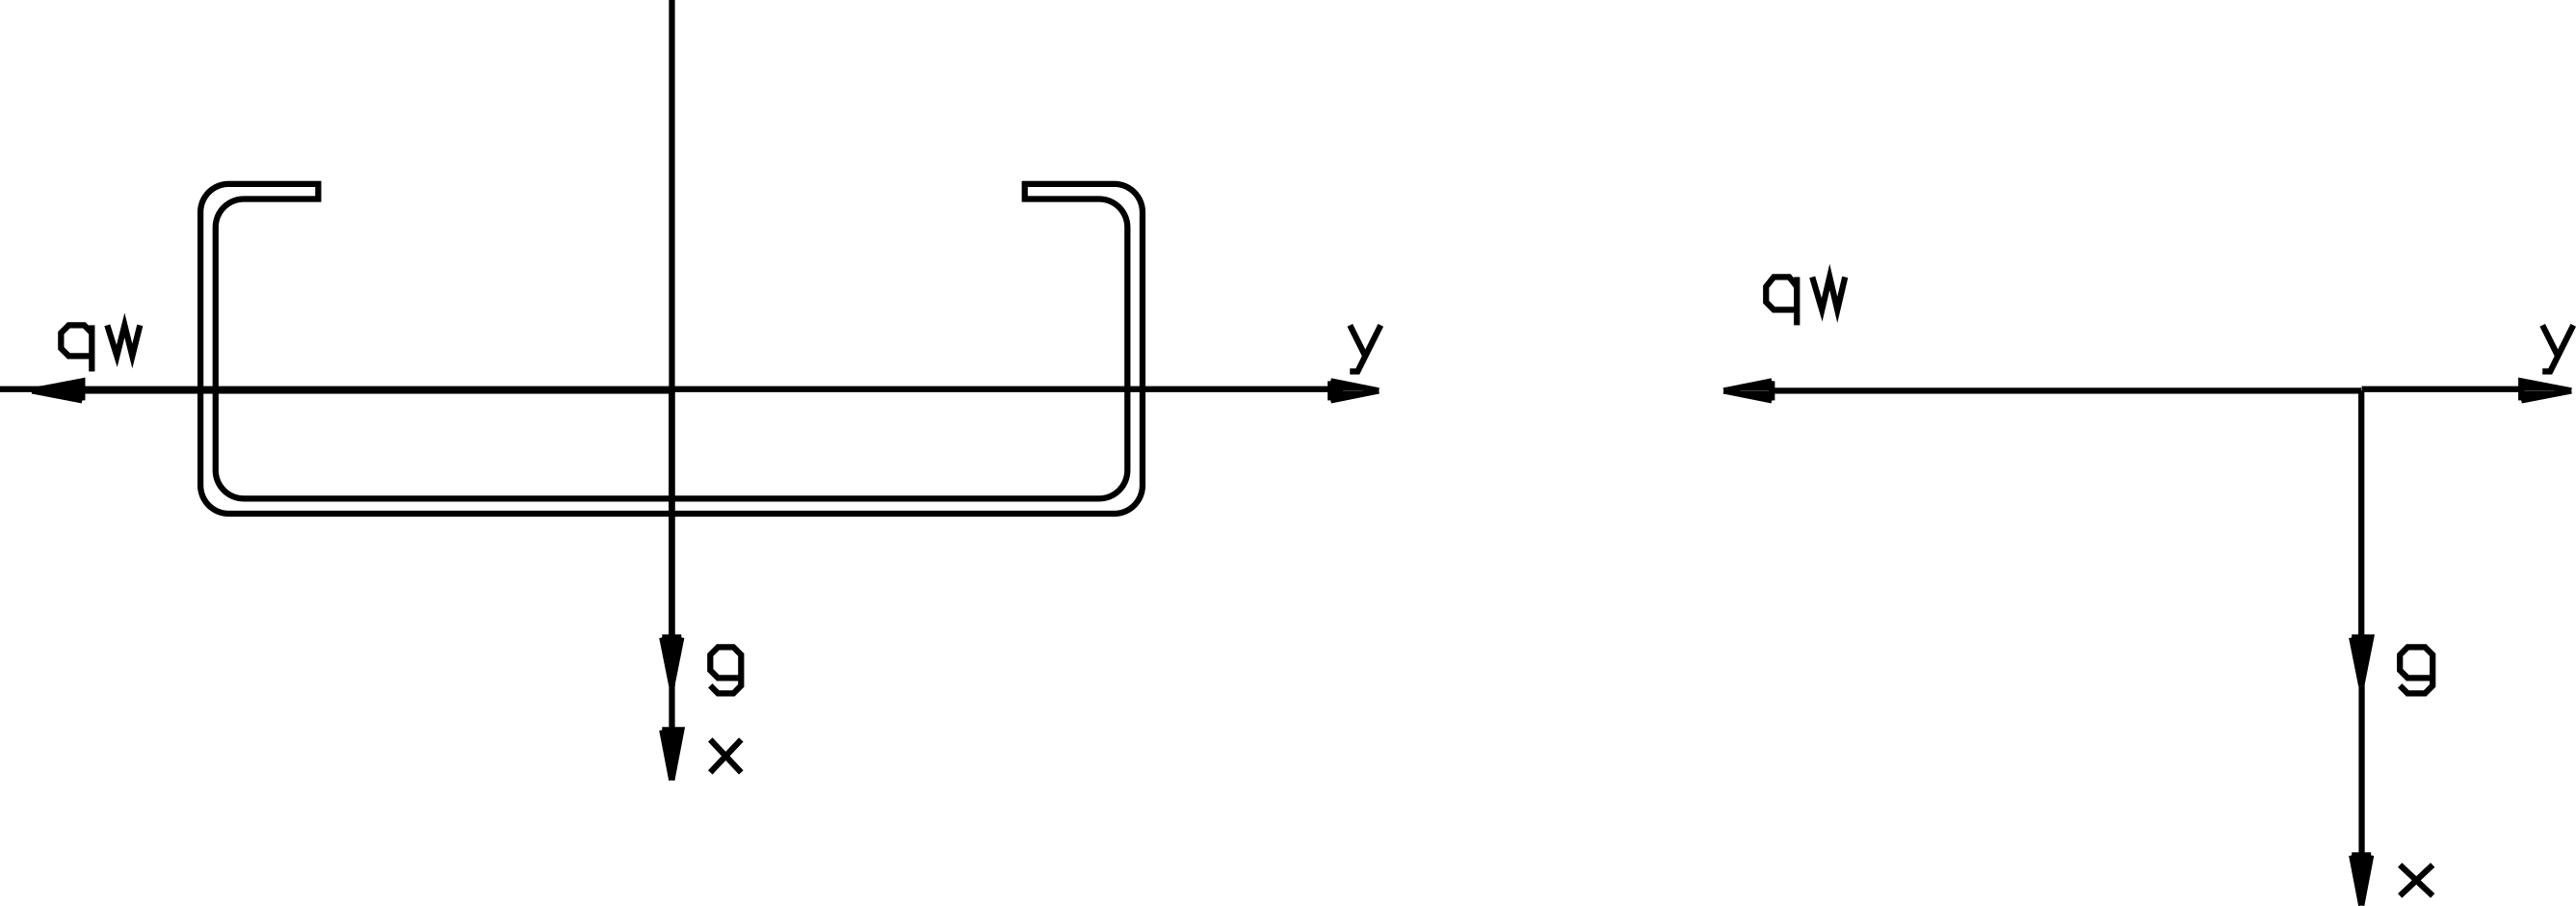
\includegraphics[scale = 1]{chapters/chapter_3/images/figura5.png}
\caption{Correa de pared - Estado: peso propio + viento}
\end{center}
\end{figure}

Descomponiendo la resultante en las direcciones $x$ e $y$ tenemos:
\begin{align*}
& \alpha = 90 \textsuperscript{o}\\
& q_x=g \cdot Sen \alpha \cdot s = 14 \frac{Kg}{m^2} \cdot 1.50m= \framebox{$21 \frac{Kg}{m}$}\\
& q_y=(q_w - g \cdot Cos \alpha) \cdot s = 150 \frac{Kg}{m^2} \cdot 1.50m= \framebox{$225 \frac{Kg}{m}$}
\end{align*}

Procedemos a calcular los momentos en el centro de la luz, producidos por cada una de estas cargas lineales, suponemos que las correas se encuentran simplemente apoyadas.

\begin{align*}
& M_x= \frac{q_y \cdot l^2}{8} = \frac{225 \frac{Kg}{m} \cdot (5m)^2}{8} = \framebox{$703.12 Kg.m$} \\
& M_y= \frac{q_x \cdot l^2}{8} = \frac{21 \frac{Kg}{m} \cdot (5m)^2}{8} = \framebox{$65.62 Kg.m$}
\end{align*}

\item Tension admisible.\\
Dado que se utiliza acero F-24, tenemos según el reglamento CIRSOC 301 una tensión de fluencia $\sigma_{fl}=2400 \frac{Kg}{cm^2}$ y tomando un coeficiente de seguridad $\gamma = 1.6$ , se obtiene una tensión admisible de:
$$\sigma_{adm}= \frac{\sigma_{fl}}{\gamma} = \frac{2400 \frac{Kg}{cm^2}}{1.6} = \framebox{$1500 \frac{Kg}{cm^2}$}$$

\item Selección de la correa.\\
Adoptamos un perfil \framebox{C 200-70-25-3.2} de chapa doblada, con las siguientes características:
\begin{align*}
& W_x= 70.448 cm^3 \\
& W_y= 16.057 cm^3 \\
& J_x= 704.478 cm^4 \\
& J_y= 78.006 cm^4
\end{align*}

\item Verificamos las tensiones para el estado de carga.\\
\underline{Estado de carga: peso propio + viento}
\begin{align*}
& \sigma_x=\frac{M_x}{W_x} = \frac{70312 Kg.cm}{70.448 cm^3} = 998.06 \frac{Kg}{cm^2}\\
& \sigma_y=\frac{M_y}{W_y} = \frac{6562 Kg.cm}{16.057 cm^3} = 408.66 \frac{Kg}{cm^2}\\
& \sigma_t= \sigma_x + \sigma_y = 998.06 \frac{Kg}{cm^2} + 408.66 \frac{Kg}{cm^2} = \framebox{$ 1406.73 \frac{Kg}{cm^2}$}\\
& \sigma_t < \sigma_{adm}\\
& 1406.73 \frac{Kg}{cm^2} < 1500 \frac{Kg}{cm^2} \Rightarrow \text{Verifica} \quad \surd
\end{align*}

\item Verificamos las deformaciones para el estado de carga.\\
La flecha admisible de cumplir $f < \frac{l}{300} \Rightarrow f < \frac{5m}{300} \Rightarrow f < 1.66cm$\\
Para el cálculo de la flecha utilizaremos la expresión $f= \frac{5}{384} \cdot \frac{q \cdot l^4}{E \cdot J}$\\

\underline{Estado de carga: peso propio + viento}
\begin{align*}
& f_x=\frac{5}{384} \cdot \frac{q_x \cdot l^4}{E \cdot J_y}\\
& f_x=\frac{5}{384} \cdot \frac{0.21 \frac{Kg}{cm} \cdot (500cm)^4}{2100000 \frac{Kg}{cm^2} \cdot 78.006 cm^4} = 1.043cm\\
& f_y=\frac{5}{384} \cdot \frac{q_y \cdot l^4}{E \cdot J_x}\\
& f_y=\frac{5}{384} \cdot \frac{2.25 \frac{Kg}{cm} \cdot (500cm)^4}{2100000 \frac{Kg}{cm^2} \cdot 704.478 cm^4} = 1.238cm\\
& f = \sqrt{f_x^2+f_y^2} = \sqrt{(1.043cm)^2+(1.238cm)^2} = \framebox{$1.62cm$}\\
& f < f_{adm}\\
& 1.62cm < 1.66cm \Rightarrow \text{Verifica} \quad \surd
\end{align*}
Por lo tanto verifica el requerimiento de deformación especificado en el reglamento.\\
\end{itemize}
\end{enumerate}
